\documentclass[dvips, a4paper, 12pt,listof=totoc, oneside, parskip]{scrbook}

\usepackage{verbatim}
\usepackage[small]{caption}
\usepackage{graphicx,psfrag}
\usepackage{rotating}
\usepackage{amsmath,amsfonts,amssymb}
\usepackage[dvips]{geometry,color}
\usepackage{xspace}
\usepackage[utf8]{inputenc}
\usepackage{wrapfig}
\usepackage{multirow}
\usepackage{placeins}

\title{Automapping rulesfile design description}
\date{Tiled v0.9}
\author{Stefan Beller}

\newcommand{\ind}{[\langle\textup{index}\rangle]}
\newcommand{\name}{\langle\textup{name}\rangle}
\begin{document}
\maketitle

\chapter*{abstract}
Automapping is an advanced tool to automatically search certain
combinations of tiles accross layers in a map and to replace
these parts by other combination. This allows the user to draw
structures with a minimum of time spent and the Automapping will be able
to generate a rather complex scenario, which would need lots more time if
manually crafted.

The first chapter of this document describes the Automapping rulemap
files in every detail.

The second chapter delivers examples which are cited by the the first part to
explain the usefulness of certain design decisions.


\chapter{Formal Description}
An automapping file consists of 4 major parts:

\begin{enumerate}
  \item The \emph{Definition of regions} describes which locations of the rulemap
  are actually used to create Automapping rules.

  \item The \emph{Definition of inputs} describes which kind of pattern the working map
  will be searched for.

  \item The \emph{Definition of outputs} describes how the working map is changed when
  an input pattern is found.

  \item The \emph{Map properties} are used to finetune the input pattern localization and the output of all rules within this rulesfile.
\end{enumerate}






\section{Defining the Regions}
There must be either a tilelayer called $\textup{regions}$ or there must be
the both tilelayers $\textup{regions}\_\textup{input}$ and
$\textup{regions}\_\textup{output}$

Using the regions layer, the region defined for input and output is
the same.

Using the different layers 'regions\_input' and 'regions\_output'
delivers the possibility to have different regions for the input section
and the output section.

The region layer(s) are only used to mark regions, where an automapping rule exists.
Therefore it does not matter which tiles are used in this layer, since these tiles are just used
to define a region.
So either use any tile or no tile at a coordinate to indicate if that coordinate belongs to a
rule or if it doesn't.

If multiple rules are defined in one rulemap file, the regions must not be
adjacent. That means there must be at least one tile of unused space in between
two rules. If the regions are adjacent (coherent) then both regions are interpreted as
one rule.

The use of different 'regions\_input' and 'regions\_output' is demonstrated
in example~\ref{example_tmw_grass_water_corners}.

\subsection{Multiple rules in one rulefile}

Of course multiple rules are possible in one rulemap.
If you want to have the rules applied in a certain sequence, you should
use multiple rulemaps and define the sequence within the rules.txt file.

As of now there also is a certain sequence within one rulemapfile.
Generally speaking the regions with small y value come first.
If there are regions at the same y value, then the x value is taken into account.
On orthogonal maps this ordering scheme is the same as for reading in most western countries.
(Left to right, top to down).

The order within one rulemap may be changed later,
once tiled is capable of utilizing multiple threads/processors.
So if you want to rely on a certain sequence, use different rulemaps and
order these in the rules.txt





\section{Definition of inputs}
Inputs are generally defined by tilelayers whichs name follows this scheme

$$\textup{input}[\textup{not}] [\langle index \rangle]  \_ \langle name \rangle$$

whereas the $[\textup{not}]$ and $[\langle index \rangle]$ are optional.

The $\langle name \rangle$ determines which layer on the working map is examined.
So for example the layer $\textup{input}\_\textup{Ground}$ will check the
layer called $\textup{Ground}$ in the working map for this rule.

Multiple layers having the same $\langle name \rangle$ and $\langle index \rangle$
is explicitly allowed and is intended. Having multiple layers of the same
$\langle name \rangle$ and $\langle index \rangle$, will allow you to define different possible tiles
per coordinate as input.

The $\langle index \rangle$ is used to create complete different input conditions.
All layers having the same $\langle index \rangle$ are taken into account for forming one
condition. Each of these conditions are checked individually.

\begin{enumerate}
  \item $\langle index \rangle$ must not contain an underscore.
  \item $\langle index \rangle$ must not start with 'not'
  \item $\langle index \rangle$ may be empty.
\end{enumerate}

If there are tiles in the standard $\textup{input}$ layers one of these tiles must be
there to match the rule. The optional $[\textup{not}]$ inverts the meaning of that layer.
So if there are $[\textup{inputnot}]$ layers, the tiles placed on them, must not
occur in the working map at the examined region to make a rule match.

Within one rule you can combine the usage of both $\textup{input}$ and $\textup{inputnot}$
layers to make rules input conditions as accurate as you need or as fuzzy
as you need.


\section{Definition of outputs}

Outputs are generally defined by tilelayers whichs name follows this scheme

$$\textup{output}[\langle index \rangle]  \_ \langle name \rangle$$

which is very similar to the input section. At first there must be the word $\textup{output}$.
Then optionally an $\textup{index}$ may occur. After the first underscore there will be the
$\textup{name}$ of the target layer.

All layers of the same index are treated as one possible output.
So the intention of indexes in the outputs of rules is only used for random
output.

The indexes in the output section have nothing to do with the indexes in the input section,
they are independant. In the output section they are used for randomness; in the input section
they are used to define multiple possible layers as input.

So when there are multiple indexes within one rule, the output will be choosen
fairly (uniformly distributed) accross all indexes. So a dice will be rolled and one index is picked.
All of the output layers carrying this index will be put out into the working map then.

Note that the output is not being checked for overlapping itself. This can be archieved by
setting the map property \emph{NoOverlappingRules} to true.




\section{Map properties}

There are 3 different map properties, which can be used to add additional
information to a rulefile:
\begin{enumerate}
  \item \emph{NoOverlappingRules}
  \item \emph{DeleteTiles}
  \item \emph{AutomappingRadius}
\end{enumerate}
These properties are map wide, meaning it applies to all rules which are part of the rulemap.
If you need rules with different properties, you can use multiple rulemaps.


\subsection{NoOverlappingRules}
A rule may not overlap to itself. It is used in example~\ref{alternatingWall}

\subsection{DeleteTiles}
This deletes all tiles in all possibly changed layers before the automapping takes place.
This is useful when using live Automapping in a map with layers, which only carry
a few tiles.

\subsection{AutomappingRadius}
Only interesting in live Automapping.

In live Automapping only a small part of the map is taken into account for Automapping to speed
up the process.
Since some rules rely on other rules to be executed first, these rules maybe should be
applied in a bigger region.

\chapter{Examples}

\newpage
\section{The Mana World examples}
%\FloatBarrier
\begin{table}
  %~ \begin{center}
        \begin{tabular}{c c}
        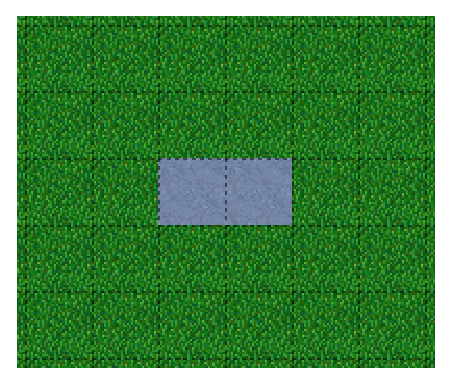
\includegraphics[scale=1]{Example/TheManaWorld/flow1.eps} &
        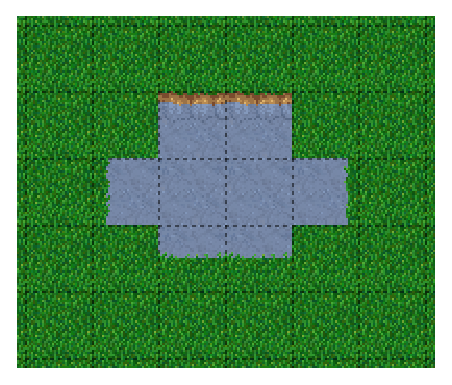
\includegraphics[scale=1]{Example/TheManaWorld/flow2.eps} \\
        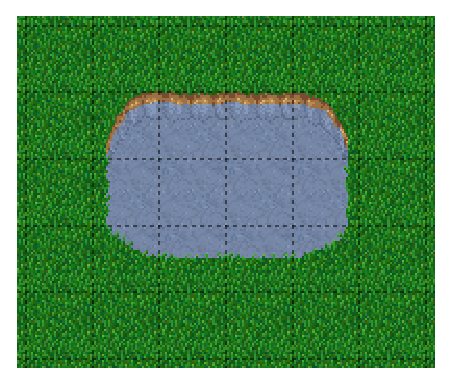
\includegraphics[scale=1]{Example/TheManaWorld/flow3.eps} &
        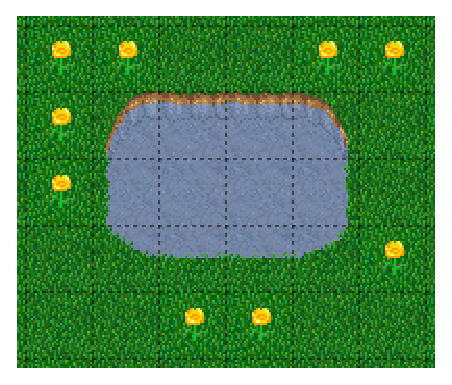
\includegraphics[scale=1]{Example/TheManaWorld/flow4.eps} \\
        \end{tabular}
  %~ \end{center}
  \caption{Series of rules get applied to build up a scenary for The Mana World. Upper left picture shows our input.
  Upper right picture shows all straigt shorelines applied. Lower left also added the bent shorelines. Lower right picture is the final version.}
\end{table}

The Mana world examples will demonstrate quite a lot of different Automapping
features. At first a shoreline will be constructed, by first adding all
the straight parts and afterwards another rule will correct the corners
to make them also fit the given tileset. After the shoreline has been added,
the waters will be marked as unwalkable for the game engine. Last but not least
some random placed fancy flowers will make the scenary even more beautiful.


\newpage
\subsection{basic shoreline} \label{basic_shoreline}
\begin{wrapfigure}{r}{0.45\textwidth}
  %~ \begin{center}
       \begin{tabular}{|c|l|}
       \hline
       tile layer & name \\
       \hline
       \hline
		
\includegraphics[scale=1]{Example/TheManaWorld/shorelinestraight/regions.eps} & regions \\
		\hline
		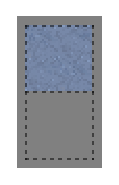
\includegraphics[scale=1]{Example/TheManaWorld/shorelinestraight/input.eps} & input\_Ground\\
		\hline
		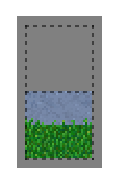
\includegraphics[scale=1]{Example/TheManaWorld/shorelinestraight/output.eps} & output\_Ground\\
		\hline
		\end{tabular}
  %~ \end{center}
  \caption{The region tile layer(top), the input tile layer(mid) and the output tile layer(bottom)}
  \label{shorelinestraight}
\end{wrapfigure}
This example will demonstrate how a straight shoreline can easily be setup 
between shallow water grass tiles. In this example we will only implement the
shoreline, which has grass in southern and water in northern direction.

So basically the meaning we will define in the input region is:
\emph{All tiles which are south of a water tile and are no water tiles itself,
will be replaced by a shoreline tile}

The region in which this Automapping rule should be defined is of 2 tiles in height and 
1 tile in width. Therefore we need a layer called \emph{regions} and it will have 2 tiles placed
to indicate this region. In figure~\ref{shorelinestraight} the top graphics shows such a region
layer.

The input layer called \emph{input\_Ground} is depicted in the middle of 
figure~\ref{shorelinestraight}. Only the upper tile is filled by the water
tile. The lower tile contains no tile. It is not an invisible tile, just no
tile at all. 

And whenever there is no tile in a place within the rule regions in an input layer,
what kind of tiles will be allowed there? There will be allowed any tiles except 
all used tiles within all input layer with the same index and name.

Here we only have one tile layer as an input layer carrying only the water tile.
Hence at the position, where no tile is located, all tiles except that water tile
are allowed.

The layer in top of 

\newpage
\subsection{Corners on a shore line}\label{example_tmw_grass_water_corners}
\begin{wrapfigure}{r}{0.6\textwidth}
  \begin{center}
		\begin{tabular}{c c c}
		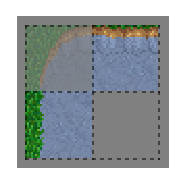
\includegraphics[scale=1]{Example/TheManaWorld/shorelinecorners/pattern0.eps} & 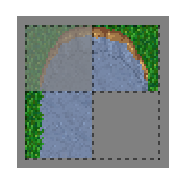
\includegraphics[scale=1]{Example/TheManaWorld/shorelinecorners/pattern1.eps} & 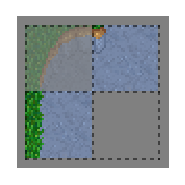
\includegraphics[scale=1]{Example/TheManaWorld/shorelinecorners/pattern2.eps} \\
		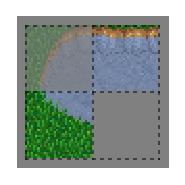
\includegraphics[scale=1]{Example/TheManaWorld/shorelinecorners/pattern3.eps} & 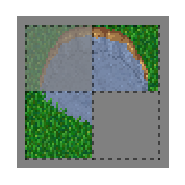
\includegraphics[scale=1]{Example/TheManaWorld/shorelinecorners/pattern4.eps} & 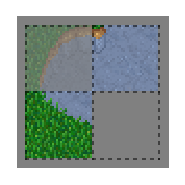
\includegraphics[scale=1]{Example/TheManaWorld/shorelinecorners/pattern5.eps} \\
		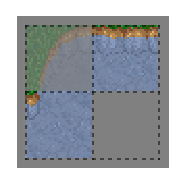
\includegraphics[scale=1]{Example/TheManaWorld/shorelinecorners/pattern6.eps} & 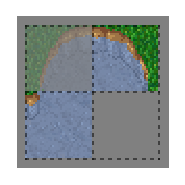
\includegraphics[scale=1]{Example/TheManaWorld/shorelinecorners/pattern7.eps} & 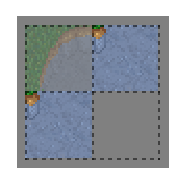
\includegraphics[scale=1]{Example/TheManaWorld/shorelinecorners/pattern8.eps} \\
		\end{tabular}
  \end{center}
  \caption{All possible inputs patterns due to other corners in the shoreline.}
  \label{shoreline_corners_needed_inputs}
\end{wrapfigure}

This example is a continuation of example~\ref{basic_shoreline}.
Now the corners of the given shoreline should be implemented automatically.
Within this paper we will just examine the bent in corner shoreline in the topleft corner.
The other shoreline corners, either bent in or bent out are constructed the same way
\footnote{Apart from some rotation and using other tiles of course.}.

So after the example~\ref{basic_shoreline} has finished, we would like to have the
corners of the shoreline get suitable tiles. Since we rely on the other example
being finished, we will put the rules needed for the corners into another new
rulefile. (which is listed afterwards in the rules.txt)

The shoreline may have some more corners nearby, which means there may be
more different tiles than the straigt corner lines. In figure~\ref{shoreline_corners_needed_inputs}
we see all inputs which should be covered.
The interesting parts are all in the red squares. Outside the red squares
it is just continued to have a niver look.

Both the tiles in the top right corner and in the lower left corner are
directly adjacent to the desired (slightly transparent) tile in the top left
corner.

We can see 3 different tiles for the lower left corner, which is
straight shore line, bent inside and bend outside shore lines.

Also we see 3 different inputs for the top right corner, which also
is straight, bent in or out shore line.

\subsubsection{regions}

\begin{wrapfigure}{r}{0.60\textwidth}
  \begin{center}
       \begin{tabular}{c c c}
		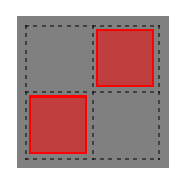
\includegraphics[scale=1]{Example/TheManaWorld/shorelinecorners/regions_input.eps} & 
		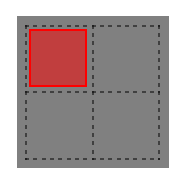
\includegraphics[scale=1]{Example/TheManaWorld/shorelinecorners/regions_output.eps} & 
		
\includegraphics[scale=1]{Example/TheManaWorld/shorelinecorners/regions_united.eps} \\
		\end{tabular}
  \end{center}
  \caption{Input regions (left) and output regions (mid) and the combination of both(right)}
  \label{shoreline_corners_regions}
\end{wrapfigure}
So with this rule we want to put the bent in shore line tile in the top
left corner, hence we don't care which tile has been there before.
Also we don't care about the tile in the lower right corner. (probably water,
but can be any decorative watertile, so just ignore it).

Therefore we will need different input and output regions. In the figure~\ref{shoreline_corners_regions}
we can see the both tilelayers $\textup{regions}\_\textup{input}$ and
$\textup{regions}\_\textup{output}$. The input section covers just these
two tiles as we discussed. The output region covers just the single tile
we want to output. Though the input and output region do not overlap,
the united region of both the input and the output region is still one coherent
region, so it's one rule and works\footnote{output regions can be larger
than absolutely required, since when there are no tiles in the output section,
the tiles in the working map are not overwritten but just kept as is, hence
the output region could also be sized as the united region of both the
output and input region.}.

\newpage
\subsubsection{input layers}
\begin{wrapfigure}{r}{0.45\textwidth}
		\begin{tabular}{|c|l|}
		\hline
		tile layer & layer name  \\
		\hline
		\hline
		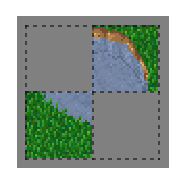
\includegraphics[scale=1]{Example/TheManaWorld/shorelinecorners/input_Ground2.eps} & input\_Ground \\
		\hline
		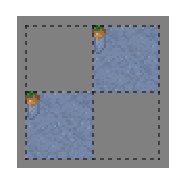
\includegraphics[scale=1]{Example/TheManaWorld/shorelinecorners/input_Ground1.eps} & input\_Ground \\
		\hline
		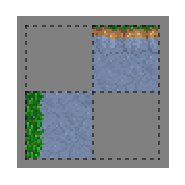
\includegraphics[scale=1]{Example/TheManaWorld/shorelinecorners/input_Ground.eps} & input\_Ground \\
		\hline	
		\end{tabular}
		\caption{All the input layer for the rule defining one corner for the shoreline.}
		\label{shorelinecorner_inputsection}		
\end{wrapfigure}
Now we want to put all the nine possible patterns we observed as possible
input for this rule. We could of course define nine different layers
$\textup{input}1  \_\textup{Ground}$ up to
$\textup{input}9  \_\textup{Ground}$
Nine TileLayers?! what a mess, we'll put it in a better way\footnote{
Also consider not having just 3 possible tiles at the 2 locations but 4.
Then we would need 4*4=16 tilelayers to get all conditions. Another downside
of this comes with more needed locations:
Think of more than 2 locations needed to construct a ruleinput. So for 3
locations, then each location could have the 3 possibilites, hence you need
3*3*3 = 27 tilelayers. It's not getting better...}


Since the rules are constructed on a per-tile basis, we only need 3 tilelayers
for the input section all of them having the same $\langle \textup{index} \rangle$,
hence the same name $\textup{input}\_\textup{Ground}$.
We need to make sure that in both positions all of each the three possible
tiles are placed. In figure~\ref{shorelinecorner_inputsection} we see the three input layers,
which match all the 9 possibilites as mentioned in figure~\ref{shoreline_corners_needed_inputs}.

\subsubsection{output}



The output is straight forward, since only one tile is needed. 
No randomness is needed, hence the $\langle \textup{index} \rangle$ is not needed to be varied, so it's kept empty.
The desired output layer is called $\textup{Ground}$, so the overall name of the single output layer
will be $\textup{output}\_\textup{Ground}$. At this single layer at the correct location the correct tile 
is placed\footnote{See top left corner in the red boxes of figure~\ref{shoreline_corners_needed_inputs}}.

\subsubsection{summary}
The table~\ref{shorelinecorner_complete} shows all layers needed for the rule, which adds corners to the shoreline in The Mana World
\begin{table}
		\begin{tabular}{|c|l|c|l|}
		\hline
		tilelayer & layer name & tilelayer & layer name\\
		\hline
		\hline
		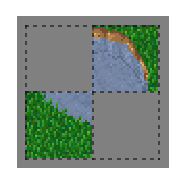
\includegraphics[scale=1]{Example/TheManaWorld/shorelinecorners/input_Ground2.eps} & input\_Ground & 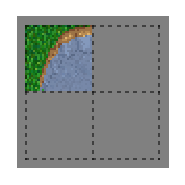
\includegraphics[scale=1]{Example/TheManaWorld/shorelinecorners/output_Ground.eps} & output\_Ground \\
		\hline
		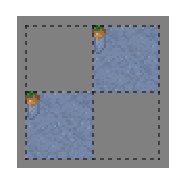
\includegraphics[scale=1]{Example/TheManaWorld/shorelinecorners/input_Ground1.eps} & input\_Ground & 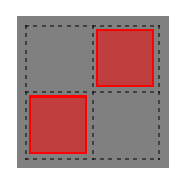
\includegraphics[scale=1]{Example/TheManaWorld/shorelinecorners/regions_input.eps} & regions\_input \\
		\hline
		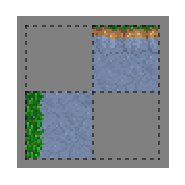
\includegraphics[scale=1]{Example/TheManaWorld/shorelinecorners/input_Ground.eps} & input\_Ground & 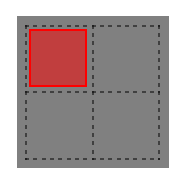
\includegraphics[scale=1]{Example/TheManaWorld/shorelinecorners/regions_output.eps} & regions\_output\\
		\hline		
		\end{tabular}
		\caption{The complete Automapping rules file defining one corner for the shoreline.}
		\label{shorelinecorner_complete}
\end{table}



\newpage
\FloatBarrier
\section{An alternating Wall} \label{alternatingWall}
\begin{table}[h!]
	\begin{tabular}{c c}
	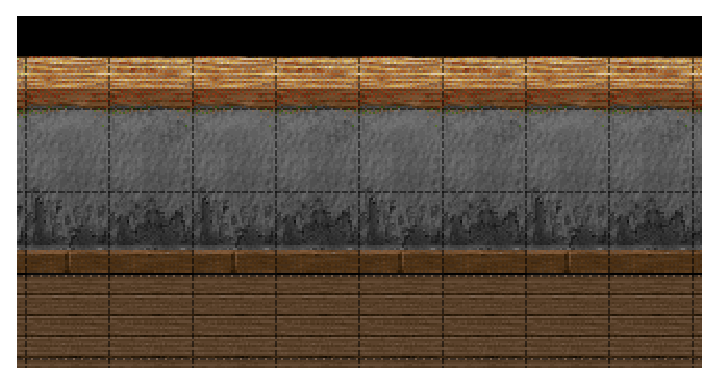
\includegraphics[scale=0.5]{Example/LoneCoder/alternatingwalls/desired.eps} &
	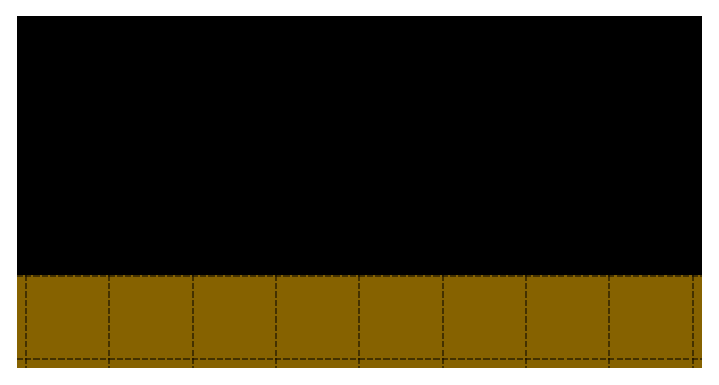
\includegraphics[scale=0.5]{Example/LoneCoder/alternatingwalls/setlayer.eps} \\
	\end{tabular}
  \caption{The left picture shows the desired wall. Vertically the tiles are alternating (Every second tile of the base board has a notch). The right picture shows the set layer.}
  \label{desiredAlternativeWall}
\end{table}

\begin{wrapfigure}{r}{0.45\textwidth}
   \begin{tabular}{|c|l|}
   \hline
   tile layer & name \\
   \hline
   \hline
	
\includegraphics[scale=0.5]{Example/LoneCoder/alternatingwalls/regions.eps} & Regions \\
	\hline
	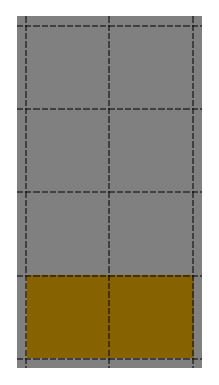
\includegraphics[scale=0.5]{Example/LoneCoder/alternatingwalls/input.eps} & Input\_set\\
	\hline
	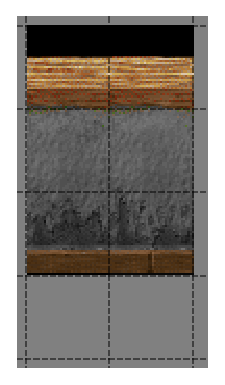
\includegraphics[scale=0.5]{Example/LoneCoder/alternatingwalls/output.eps} & Output\_Walls\\
	\hline
	\end{tabular}
  \caption{The region tile layer(top), the input tile layer(mid) and the output tile layer(bottom)}
  \label{alternatingWallsRule}
\end{wrapfigure}

This example will demonstrate how a wall as a transition between a walkable 
area and the nonwalkable black void can easily be setup. 
As input a dedicated set layer will be used.

The structure of the input, output and region layer is very similar to the example~\ref{basic_shoreline}.
The main difference is the different size. Since the wall contains multiple tiles in height,
the height of the rulelayers is different as well. Vertically the tiles are also alternating. 
As you can see in figure~\ref{desiredAlternativeWall}, every second tile displaying the base board of the Wall has a notch for example.

Hence the region in which this Automapping rule should be defined is of 4 tiles in height and 
2 tile in width. Therefore we need a layer called \emph{Regions} and it will have 8 tiles placed
to indicate this region. In figure~\ref{alternatingWallsRule} the top graphics shows such a region
layer.

The input layer has the following meaning: \emph{If there are 2 vertical adjacent brown tiles in the set layer
and in the 3x2 tiles above there are no brown tiles, this rule matches.}
Only the lowest 2 coordinates contain the brown tile. The upper coordinates contains no tile. 
(It is not an invisible tile, just no tile at all.)
The input layer called \emph{Input\_set} is depicted in the middle of 
figure~\ref{alternatingWallsRule}. 

The output consists of only one layer as well called \emph{Output\_Walls}.
It contains the actual wall tiles.

When trying to match the input layer to the desired set layer (right picture of figure~\ref{desiredAlternativeWall},
you will see it matches all way long, no matter of the vertical adjustment.

Hence when we use the rule as discussed now, we will get not the desired result, but this rule
overlaps itself. The overlapping problem is shown in figure~\ref{problemAlternativeWall}

\begin{table}
	\begin{tabular}{c c}
	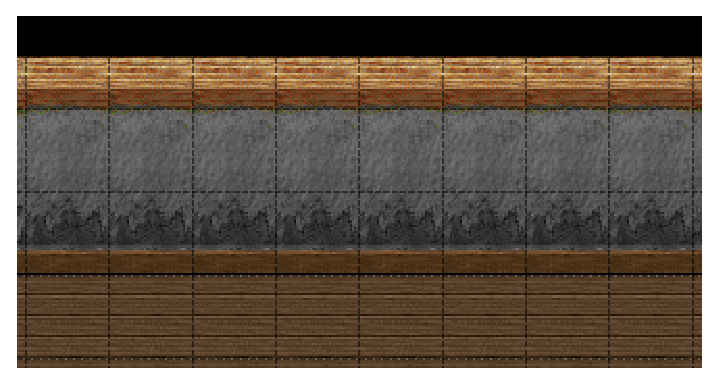
\includegraphics[scale=0.5]{Example/LoneCoder/alternatingwalls/firstattempt.eps} &
	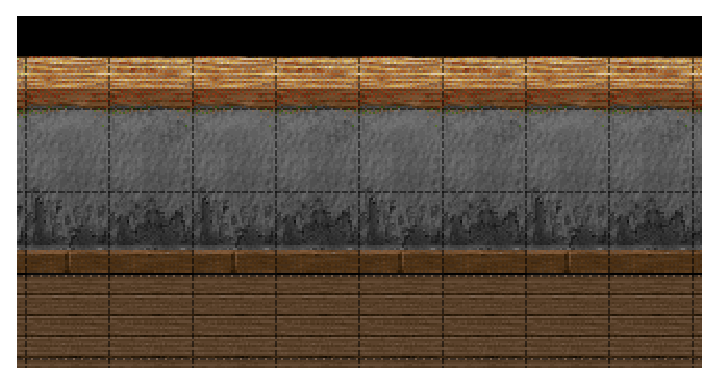
\includegraphics[scale=0.5]{Example/LoneCoder/alternatingwalls/desired.eps} \\
	\end{tabular}
  \caption{The left picture shows the first attempt of the wall. Only the first parts of the wall is created, 
  the second parts have been overwritten by another instance of this rule.
  The right picture shows the correct version by setting the map property \emph{NoOverlappingRules} to true.}
  \label{problemAlternativeWall}
\end{table}

Since the overlapping is not desired, we can turn it off by adding a map property to the rulemap
\emph{NoOverlappingRules} and setting it to "true".

Mind, that the map property applies for all rules on that rule map.





\newpage
\section{abstract input layer examples}
\subsection{having multiple input layers with the same name}
Assume the following 3 tile layers as input, which possible inputs are there in the working map?
\begin{table}[h!]
        \begin{tabular}{|c|l|}
        \hline
		tile layer & name \\
        \hline
        \hline
		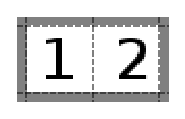
\includegraphics[scale=1]{Example/AbstractInput/12.eps} & input\_Ground \\
		\hline
		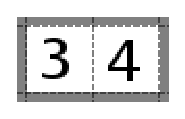
\includegraphics[scale=1]{Example/AbstractInput/34.eps} & input\_Ground\\
		\hline
		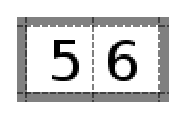
\includegraphics[scale=1]{Example/AbstractInput/56.eps} & input\_Ground\\
		\hline
		\end{tabular}
\end{table}

The following parts would be detected as matches for this rule:
\begin{table}[h!]
        \begin{tabular}{c c c}
		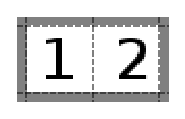
\includegraphics[scale=1]{Example/AbstractInput/12.eps} & 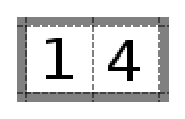
\includegraphics[scale=1]{Example/AbstractInput/14.eps} & 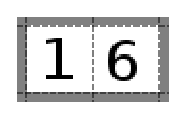
\includegraphics[scale=1]{Example/AbstractInput/16.eps} \\
		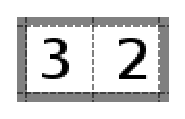
\includegraphics[scale=1]{Example/AbstractInput/32.eps} & 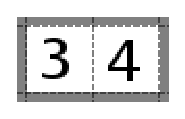
\includegraphics[scale=1]{Example/AbstractInput/34.eps} & 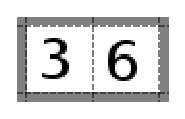
\includegraphics[scale=1]{Example/AbstractInput/36.eps} \\
		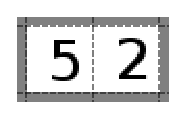
\includegraphics[scale=1]{Example/AbstractInput/52.eps} & 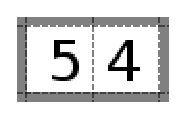
\includegraphics[scale=1]{Example/AbstractInput/54.eps} & 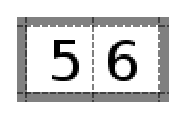
\includegraphics[scale=1]{Example/AbstractInput/56.eps} \\
		\end{tabular}
\end{table}

\newpage
\subsection{input layers using different indexes}
Given the following 3 input tile layers:
\begin{table}[h!]
        \begin{tabular}{|c|l|}
        \hline
		tile layer & name \\
        \hline
        \hline
		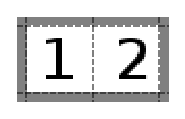
\includegraphics[scale=1]{Example/AbstractInput/12.eps} & input\_Ground \\
		\hline
		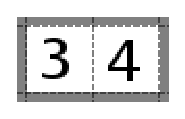
\includegraphics[scale=1]{Example/AbstractInput/34.eps} & input\_Ground\\
		\hline
		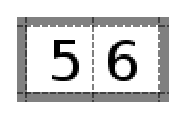
\includegraphics[scale=1]{Example/AbstractInput/56.eps} & input2\_Ground\\
		\hline
		\end{tabular}
\end{table}

All following parts would be recognized as matches within the working map:
\begin{table}[h!]
        \begin{tabular}{c c c}
		\includegraphics[scale=1]{Example/AbstractInput/12.eps} & \includegraphics[scale=1]{Example/AbstractInput/14.eps} & \\
		\includegraphics[scale=1]{Example/AbstractInput/32.eps} & \includegraphics[scale=1]{Example/AbstractInput/34.eps} & \includegraphics[scale=1]{Example/AbstractInput/56.eps} \\
		\end{tabular}
\end{table}


\chapter{Hints}

dedicated set layer or trying to parse your layer

\end{document}
